\documentclass[titlepage]{article}
\usepackage{tikz}
\usepackage{enumerate}
\usepackage{amsmath}
\usetikzlibrary{arrows,automata}
\begin{document}
\title{TDT4205 Compiler Technology Problem Set 1}
\maketitle
\setcounter{secnumdepth}{0}

\section{Problem 1}
gcc: (Ubuntu/Linaro 4.6.3-1ubuntu5) 4.6.3\\
flex: 2.5.35\\
bison:(GNU Bison) 2.5\\

\section{Problem 2}
Compilers translate source code into executable machine code which may then be executed by separate commands, whereas an interpreter translates and executes one statement at a time. As a result, compilers perform a great deal more preprocessing than an interpreter.

\section{Problem 3}
\begin{enumerate}[a)]
\item \leavevmode{\vspace{-\baselineskip}}\\
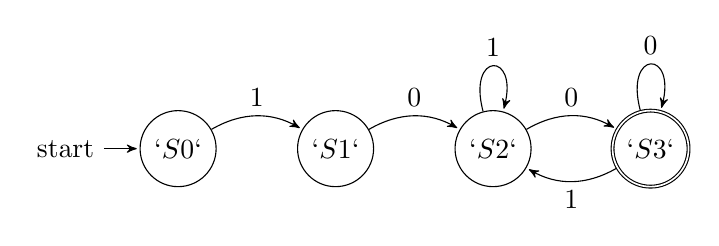
\begin{tikzpicture}[>=stealth',shorten >=1pt,auto,node distance=2cm]
  \node[initial,state] (S)      {`$S0$`};
  \node[state]         (q1) [right of=S]  {`$S1$`};
  \node[state]         (q2) [right of=q1] {`$S2$`};
  \node[state,accepting]         (q3) [right of=q2] {`$S3$`};

  \path[->] (S)  edge [bend left] node {1} (q1)
        (q1) edge [bend left]  node {0} (q2)
        (q2) edge [bend left]  node {0} (q3)
             edge [loop above] node {1} (q2)
             (q3) edge [loop above] node {0} (q3)
             edge [bend left]  node {1} (q2);
\end{tikzpicture}
\item
The language includes even binary numbers $\ge$ 4, e.g. 100, 10100 or 1010101110001010010010110
\item
\begin{tabular}{c c|c}
current state & input & next state\\
\hline
S0 & 1 & S1\\
S1 & 0 & S2\\
S2 & 0 & S3\\
S2 & 1 & S2\\
S3 & 0 & S3\\
S3 & 1 & S2\\
\end{tabular}
\end{enumerate}

\section{Problem 4}

\end{document}
